\documentclass[12pt]{amsart}
\usepackage[english]{babel}
\usepackage[left=0.75in, right=0.75in, bottom=0.75in, top=0.75in]{geometry}
\usepackage[utf8x]{inputenc}
\usepackage{amsmath,amssymb,amsthm}
\usepackage{enumerate}
\usepackage{graphicx}
\usepackage{booktabs}

\usepackage[table,dvipsnames]{xcolor}
\usepackage{caption}
\usepackage{pgf,tikz,tikz-3dplot}
\usetikzlibrary{shapes,arrows,positioning,backgrounds}
\tikzset{%
	goodnode/.style={circle, draw=MidnightBlue!90, thick, fill=gray!40},
	okaynode/.style={circle, draw=Orange!90, thick, fill=gray!40},
	badnode/.style={circle, draw=Red!90, thick, fill=gray!40},
	togood/.style={draw=MidnightBlue, thick,->,>=stealth',shorten >=1pt},
	tookay/.style={draw=Orange, thick,->,>=stealth',shorten >=1pt},
	tobad/.style={draw=Red, thick,->,>=stealth',shorten >=1pt}}

\usepackage{float}

\title{OPER 640 - Stochastic Modeling and Analysis}
\author{B. Hosley}
\date{\today}

\begin{document}
	\maketitle
	\raggedbottom

\section{Description}

% Problem description
% 	Paraphrase project description,
% 	formulate analysis questions of interest to leadership

\subsection{The current situation}

After arriving to the data masked location regeneration efforts have begun 
for all aircraft assigned to the squadron.
Three aircraft are undergoing a final inspection and, pending results of that inspection,
will be cleared to fly by the next ATO cycle.
The remaining nine aircraft are undergoing restoration for flight conditions after travel,
Three will finish each ATO cycle for the next three cycles and, pending need
for additional unplanned maintenance, will also be cleared for operation.

\subsection{Purpose of this report}

The purpose of this report is to provide the technical background requested by leadership
supporting the recommendations provided in a previous report.
To this end it will provide information regarding the expected numbers of fully mission 
capable aircraft available for sortie generation, and how these estimations were determined.
Provided the intent is met, it will provide greater confidence in the information
provided to decision makers to make and take more informed courses of action.

\subsection{Initial inquiries}

First, we will examine the expected time it will take, starting from the 
current situation, for the squadron to return to sortie generating capable.
Second, we will examine the expected long term availability of aircraft
if the current operational conditions persist.
Finally, we will examine the effects of changes to current operations, 
to provide the information necessary to evaluate which of those changes 
will have the greatest return on investment.


\section{Modeling the Situation}

\subsection{Model Specifications}

Based on the information provided, this system will lend itself well to being modeled 
by a discrete-time Markov chain.
This system will be represented as \(\{X_n : n\geq0\}\) where 
\(X_n = \{X_n^1,X_n^2,X_n^3,X_n^4,X_n^5\}\) such that
\(X_n^i\) represents the number of aircraft in condition \(i\) at time \(n\).
Each of the conditions \(i\) are classified explicitly in Table \ref{states}. \\

\begin{table}[H]
	\begin{tabular}{rcl}
		\toprule
		\(i\) & & \textit{Condition Description} \\
		\midrule
		1 & FMC & Fully mission capable \\
		2 & FS  & In the front shop for inspection or minor repair \\
		3 & BS1 & First ATO cycle in backshop \\
		4 & BS2 & Second ATO cycle in backshop \\
		5 & BS3 & Last ATO cycle in backshop \\
		\bottomrule
	\end{tabular}
	\caption{Aircraft States.}
	\label{states}
\end{table}

\subsubsection{State Space}

The state space, or the list of every possible configuration of this model is every
combination of aircraft in each condition.
Further, in adherence to standardization we have relied on the perfect interchangeability 
of each aircraft, as a result each state concerns only how many aircraft are in each condition,
and does not make any distinctions regarding which specific aircraft comprise the count.
Therefore, the state space is comprised of every combination of aircraft in each of the
conditions such that
\begin{align}
	\sum_{i=1}^{5}X_n^i = 12.
\end{align}

The state space will not be further enumerated here, analytically the 
number of unique states is a multiset which can be calculated as
\begin{align}
	\left( \hspace{-0.4em} \binom{5}{12} \hspace{-0.4em} \right) 
	=\binom{5+12-1}{12}
	=\frac{16!}{12!\ 4!}
	= 1820
\end{align}
distinct states.

For the sake of brevity we will generally focus only on the states in which
\(X_n^1\geq8\) representing the ATO cycles where the minimum aircraft
needed to meet the sortie requirement are operationally capable.
Within this state space there are 70 such states,

\subsubsection{Markov Property}

Remarkably, the data show that there is no correlation between past failed
inspections or major maintenance and future occurrences of the same.
The maintainers of this squadron are so skilled it is as if the 
aircraft have no memory of past conditions.
This observation is extremely significant as it simplifies the manner 
in which we can model the expected conditions of the aircraft in the squadron.

\subsubsection{Time Homogeneity}

The strict adherence to doctrine and training has made it such that 
even in the face of significant unpredictability,
the squadron's maintainers perform their work with the exact
same quality in each ATO cycle.
Consequently, the changes to the condition of each aircraft have the 
same probability between each ATO cycle. 
For example, after every sortie completed there is a 20\% chance that
the aircraft will need to undergo inspection, and during each 
cycle in which an aircraft undergoes inspection and minor repairs
it is cleared to fly in the next ATO 70\% of the time, every time.

\subsubsection{Transition Probability}



% Construct the Transition Probability Matrix. Or specify probability function p_ij.


Figure \ref{DTMC} shows the state-cycle of an individual aircraft.

\begin{figure}[H]
	\centering
	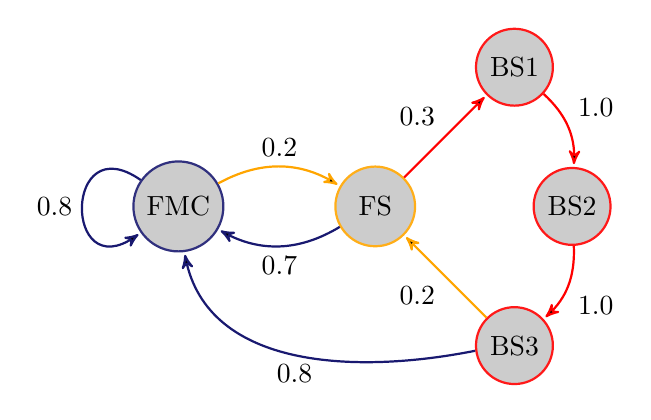
\begin{tikzpicture}[node distance=2.5cm]		
		\node[goodnode] (FMC) {FMC};
		\node[okaynode] (FS) [right of=FMC] {\(\ \)FS\(\ \)};
		\node[badnode] (BS1) [above right of=FS] {BS1};
		\node[badnode] (BS2) [right of=FS] {BS2};
		\node[badnode] (BS3) [below right of=FS] {BS3};
		
		\path[togood] (FMC) 	edge [loop left, min distance=12mm, out=145, in=215]  node [left] 	{\(0.8\)} (FMC);
		\path[togood] (FS)  	edge [bend left]  node [below] 	{\(0.7\)} (FMC);
		\path[togood] (BS3) 	edge [bend left, in=120]  node [below] 	{\(0.8\)} (FMC);
		
		\path[tookay] (FMC) 	edge [bend left]  node [above] 	{\(0.2\)} (FS);
		\path[tookay] (BS3) 	edge []  node [below left] 	{\(0.2\)} (FS);
		
		\path[tobad]  (FS) 		edge []  node [above left] 	{\(0.3\)} (BS1);
		\path[tobad]  (BS1) 	edge [bend left=25]  node [above right] 	{\(1.0\)} (BS2);
		\path[tobad]  (BS2) 	edge [bend left=25]  node [below right] 	{\(1.0\)} (BS3);
	\end{tikzpicture}
	\caption{Single Entity DTMC.}
	\label{DTMC}
\end{figure}



\section{Baseline Analysis}

% Baseline analysis - primary analysis questions
% 	How often will the squadron be able to achieve mission success, meeting 8-orbit mission requirements
% 	How long will it take for the squadron become FMC >= 8 aircraft
% 	What is the long-term sortie generation rate?
% 	What is the long-term mission capable aircraft availability rate?

\begin{figure}
	\centering
	\includegraphics[width=0.7\linewidth]{Images/baseline}
	\caption{}
	\label{fig:baseline}
\end{figure}


\section{Exploratory Analysis}

% Sensitivity (excursion) analyses - the what-if questions, 
% 	explore possible solutions by modifying parameter values


\begin{figure}
	\centering
	\includegraphics[width=0.7\linewidth]{Images/BackshopImpairment}
	\caption{}
	\label{fig:backshopimpairment}
\end{figure}
\begin{figure}
	\centering
	\includegraphics[width=0.7\linewidth]{Images/BackshopImprovement}
	\caption{}
	\label{fig:backshopimprovement}
\end{figure}

\begin{figure}
	\centering
	\includegraphics[width=0.7\linewidth]{Images/FrontShopImpairment}
	\caption{}
	\label{fig:frontshopimpairment}
\end{figure}
\begin{figure}
	\centering
	\includegraphics[width=0.7\linewidth]{Images/FrontShopImprovement}
	\caption{}
	\label{fig:frontshopimprovement}
\end{figure}

\begin{figure}
	\centering
	\includegraphics[width=0.7\linewidth]{Images/PostflightImpairment}
	\caption{}
	\label{fig:postflightimpairment}
\end{figure}
\begin{figure}
	\centering
	\includegraphics[width=0.7\linewidth]{Images/PostflightImprovement}
	\caption{}
	\label{fig:postflightimprovement}
\end{figure}


\begin{figure}
	\centering
	\includegraphics[width=0.7\linewidth]{Images/DecreasedSortieRequirement}
	\caption{}
	\label{fig:decreasedsortierequirement}
\end{figure}
\begin{figure}
	\centering
	\includegraphics[width=0.7\linewidth]{Images/AdditionalAircraft}
	\caption{}
	\label{fig:additionalaircraft}
\end{figure}




\section{Conclusions and Recommendations}

% Conclusions and recommendations


\end{document}